\documentclass[12pt, a4paper, hidelinks, svgnames]{article}
\usepackage{natbib} 
\usepackage{amsmath}  % Necesario para usar subequations
\usepackage{multirow}
\usepackage{colortbl}
\usepackage{amsmath}  % Para ecuaciones
\usepackage{adjustbox}  % Para ajustar el tamaño de la tabla
\usepackage{graphicx}   % Para el entorno table si es necesario
\usepackage{booktabs}   % Para líneas horizontales más claras
\usepackage[table,xcdraw]{xcolor}
\usepackage{graphicx}
\usepackage{subcaption}

\usepackage{array} % Para centrar las celdas
\renewcommand{\arraystretch}{1.5} % Aumentar la altura de las filas

%% PACKAGES
% Packages Information: https://www.ctan.org/pkg

% Language
\usepackage[brazil]{babel}
\usepackage[utf8]{inputenc}

% Page formating
\usepackage[left=30mm, right=20mm, top=30mm, bottom=20mm]{geometry}
\usepackage[toc,page, title, titletoc]{appendix}

% Tables
\usepackage[table,xcdraw]{xcolor}
\usepackage{booktabs}
\usepackage{multicol}
\usepackage{multirow}

% Figures
\usepackage{graphicx}
\usepackage{adjustbox}
\usepackage{caption}
\usepackage{subcaption}
\usepackage{float}
\usepackage{pgfplots}
\pgfplotsset{compat=1.16}

% Colors
\usepackage{xcolor}

% Math
\usepackage{mathtools}
\usepackage{amssymb}
\usepackage{amsfonts}
\usepackage{xfrac}
\newtheorem{theorem}{Teorema}

% Text formatting
\edef\svtheparindent{\the\parindent}
\usepackage{parskip}
\parindent=\svtheparindent\relax
\usepackage{indentfirst}
\usepackage{microtype}
\usepackage{titlesec}
\usepackage{hyperref}
\usepackage{setspace}
\usepackage{soul}

\titleformat*{\section}{\large\bfseries}
\titleformat*{\subsection}{\normalsize\bfseries}
\titleformat*{\subsubsection}{\normalsize\it}
\titleformat*{\paragraph}{\normalsize\it}
\titleformat*{\subparagraph}{\normalsize\it}

% Fonts
\usepackage{lipsum}
\usepackage[T1]{fontenc}
%\usepackage{libertine}
%\usepackage{libertinust1math}
%\usepackage[T1]{fontenc}
%\renewcommand*\familydefault{\sfdefault}


\begin{document}

\begin{titlepage}
\begin{center}
\textbf{UNIVERSIDADE DE SÃO PAULO - USP\\
ESCOLA DE ENGENHARIA DE SÃO CARLOS\\
DEPARTAMENTO DE ENGENHARIA AERONÁUTICA}\\[2cm]

\large Geovana Zanati - nº USP: 11917434\\
\large Joel Riascos - nº USP: 15515332\\
\large Gabriel Delgado Albuquerque - nº USP: 11857365\\

\hfill\break
\hfill\break
\hfill\break
\hfill\break
\hfill\break

\huge{\textbf{Ensaios em túnel de vento de um cilindro, uma seção e uma asa tridimensional}}\\
%\Large{Subtítulo}
\vspace{5cm}

\normalsize{PROFESSOR \MakeUppercase{Fernando Martini Catalano}}\\
\normalsize{PROFESSOR \MakeUppercase{Hernan Dario Ceron Muñoz}}\\
\normalsize{Disciplina: SAA0198 - Métodos Experimentais em Aerodinâmica}

\vfill
\large \textbf{São Carlos - SP}\\
\large \textbf{\today}\\
\end{center}
\end{titlepage}

\tableofcontents
\clearpage
\listoffigures
\listoftables
%\section{Resumo}

\section{Introdução}
O presente trabalho apresenta os resultados dos experimentos realizados nos túneis de vento da universidade para a disciplina "Métodos Experimentais em Aerodinâmica" do curso de graduação em Engenharia Aeronáutica. 

O primeiro experimento realizado pelo grupo consistiu na análise dos valores de coeficiente de pressão em pontos superficiais ao longo de uma seção transversal de um cilindro posicionado paralelamente à direção do escoamento no interior do túnel de vento, considerando-se como uma configuração 2D. 

O segundo experimento foi o ensaio de uma asa em configuração para análise de aerodinâmica bidimensional dos coeficientes de sustentação, de arrasto e de momento. 

O terceiro, por sua vez, tratou-se do ensaio da asa em configuração para análise da aerodinâmica tridimensional, também com cálculos de coeficientes de sustentação, de arrasto e de momento. 

Os ensaios se inserem no contexto de introdução a métodos experimentais em aerodinâmica aos alunos e objetivam o ensino de boas práticas no uso dos instrumentos, bem como validação de conceitos básicos aprendidos via aerodinâmica analítica. 

\section{Desenvolvimento}
%Escrever um desenvolvimento comum aos três experimentos
%Colocar dimensões e parâmetros do túnel (lembrar dos coeficientes KL e KM), talvez já com as dimensões dos objetos de ensaio

\subsection{Cálculo de coeficientes de pressão no cilindro}

% Anteriormente ao início da coleta de dados, verificou-se a adequada instalação do cilindro e do tubo de Pitot na câmara de ensaio, conforme determinam as boas práticas para um procedimento efetivo. O cilindro possui um orifício, no qual a tomada de pressão ao longo do experimento é realizada. Configura-se o cilindro na posição inicial correspondente a 0° (ângulo entre a direção axial do orifício e a direção vertical). 

% Os terminais de um micromanômetro foram conectados à tomada de pressão estática local e ao tubo de Pitot, para assim retornar o cálculo diferencial entre as pressões estáticas local e do escoamento livre correspondente a cada ponto de ensaio. Ligou-se então o túnel e se iniciou a coleta de valores de pressão dinâmica para valores graduais de rotação do cilindro, de 0° (valor inicial) a 180°. Considerando a simetria axial do cilindro, este conjunto de dados é suficiente para se determinar resultados para toda posição do orifício ao redor da seção transversal do objeto de ensaio. Entre 180° e 360°, a curva deve convergir e se estabilizar, pois o orifício se encontra obstruído pelo cilindro em relação à direção do escoamento.

% Seguiu-se então para o cálculo dos coeficientes de pressão a partir dos valores de pressão dinâmica coletados. Como na configuração inicial do cilindro a posição do orifício coincide com o ponto de sucção, o valor obtido pelo micromanômetro nesta medida é por definição igual à tomada de pressão dinâmica do escoamento livre. Assim, cada coeficiente de pressão se dá pela divisão entre o dado coletado no ponto em cada medida e o dado coletado no ponto inicial. 
Antes de iniciar a coleta de dados, foi verificada a instalação adequada do cilindro e do tubo de Pitot na câmara de ensaio, seguindo boas práticas. O cilindro possui um orifício para medição de pressão e é posicionado inicialmente a 0° em relação à vertical. Os terminais de um micromanômetro foram conectados para calcular a diferença entre as pressões estáticas local e do escoamento livre. Após ligar o túnel de vento, foram coletados dados de pressão dinâmica variando a rotação do cilindro de 0° a 180°. Devido à simetria axial do cilindro, esses dados são suficientes para determinar os resultados para toda a seção transversal do objeto. Entre $180^\circ$ e $360^\circ$, a curva deve convergir e estabilizar, pois o orifício fica obstruído pelo cilindro em relação ao escoamento.

Em seguida, foram calculados os coeficientes de pressão a partir dos valores de pressão dinâmica coletados. Na configuração inicial, a posição do orifício coincide com o ponto de sucção, tornando o valor obtido pelo micromanômetro igual à pressão dinâmica do escoamento livre. Cada coeficiente de pressão é obtido dividindo o dado coletado em cada medição pelo dado do ponto inicial.

\begin{figure}[htbp]
    \centering
    \begin{subfigure}{0.35\textwidth}
        \centering
        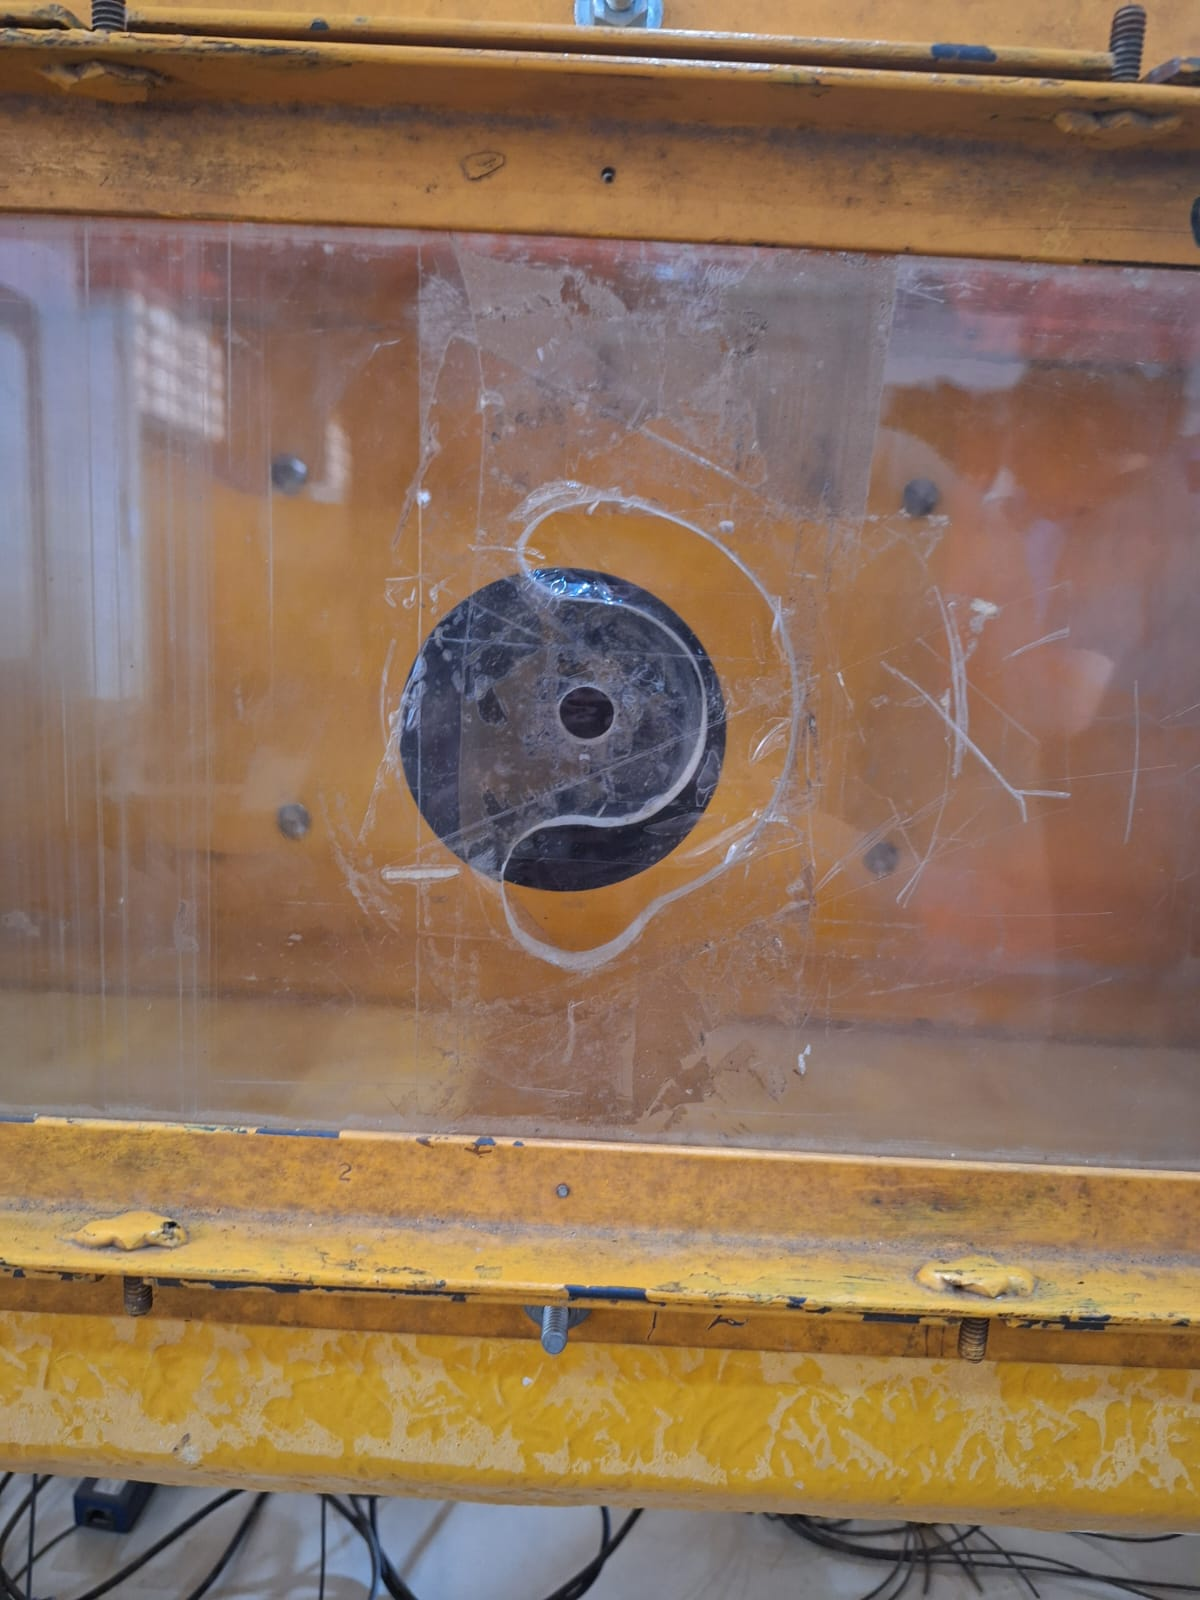
\includegraphics[width=\textwidth]{01.Parte1/Figuras/Cilindro - representação - vista da seção.jpg}
        \caption{Seção transversal do cilindro}
        \label{fig:SecTrans}
    \end{subfigure}
    \hfill
    \begin{subfigure}{0.55\textwidth}
        \centering
        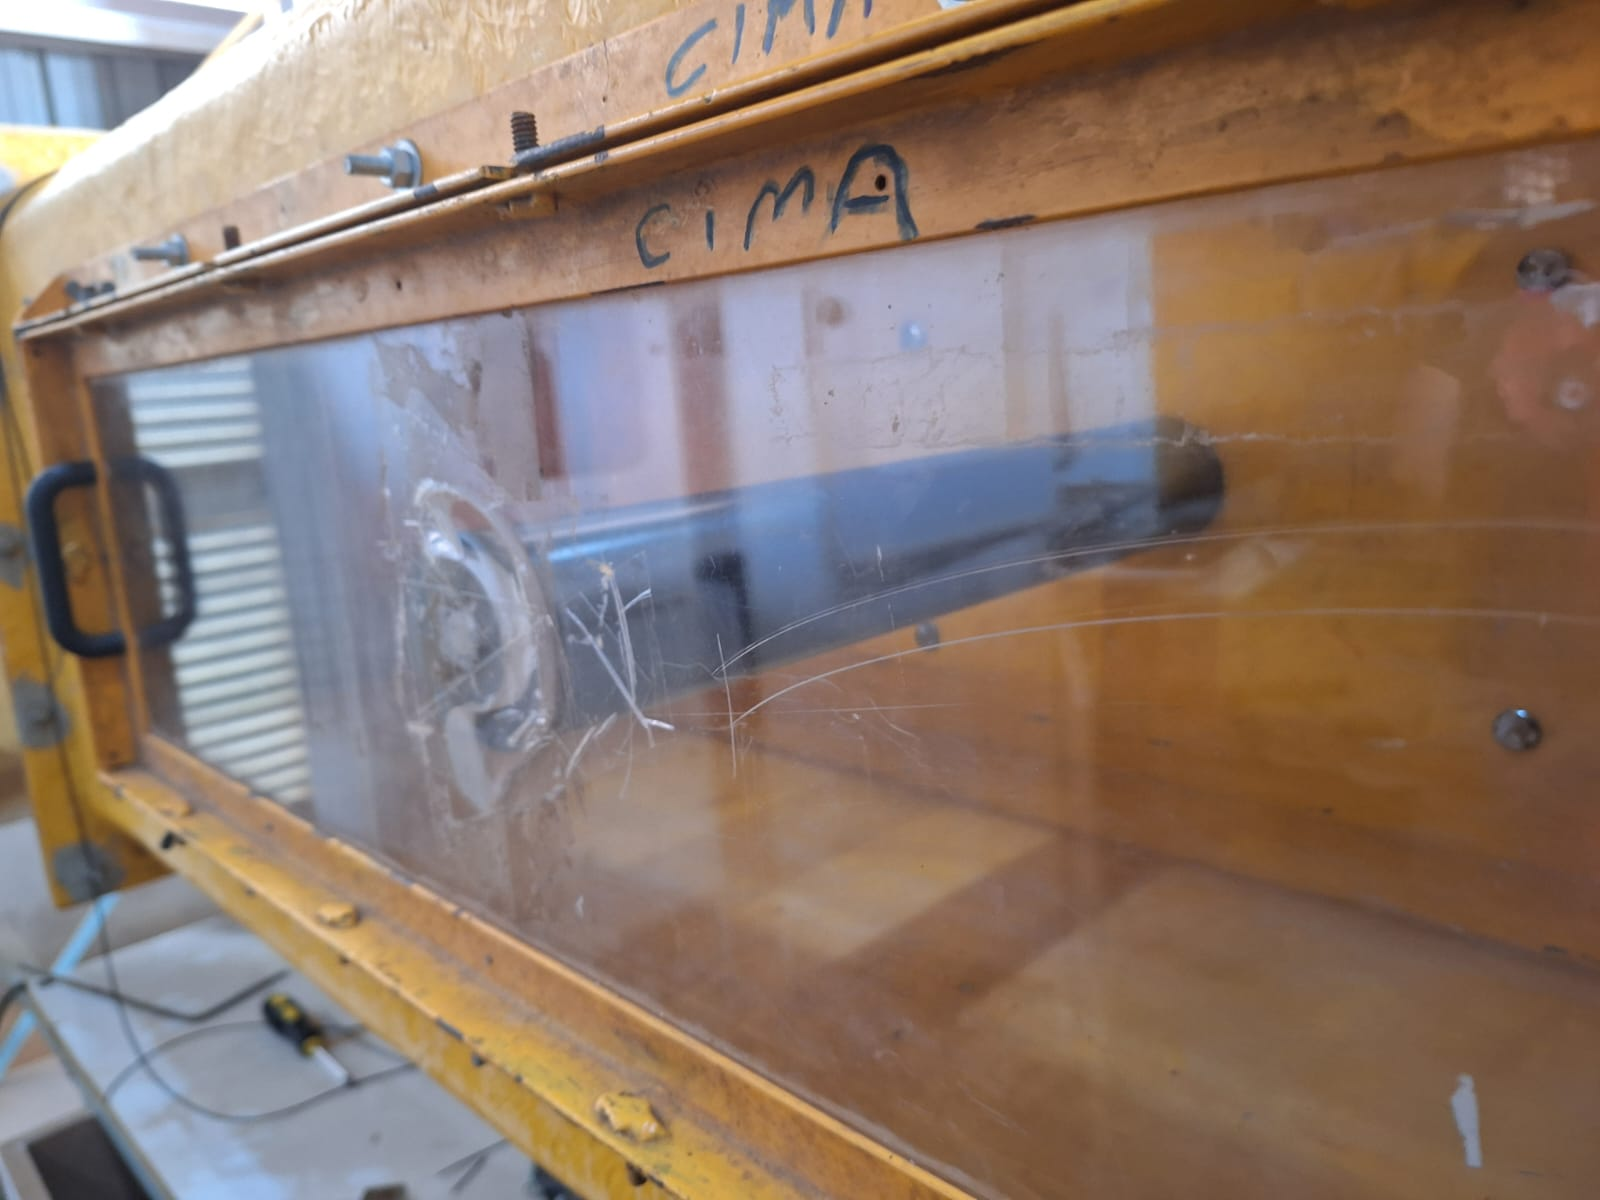
\includegraphics[width=\textwidth]{01.Parte1/Figuras/Cilindro - representação - vista em perspectiva.jpg}
        \caption{Montagem do cilindro no túnel de vento}
        \label{fig:Monta}
    \end{subfigure}
    
    \caption{Experimento de cilindro liso}
    \label{fig:dos_imagenes}
\end{figure}

Também foram calculados calculadas as seguintes variáveis e seus respectivos erros:
\begin{itemize}
    \item A densidade do ar
    \item Velocidade do escoamento livre
    \item Viscosidade dinâmica do ar
    \item Número de Reynolds
    \item Mach
\end{itemize}

Obtida das medidas de $C_p$, a Figura \ref{fig:Cp} mostra a comparação entre o coeficiente de pressão obtido no experimento e o coeficiente de pressão potencial (teórico).

Primeiramente, o método de cálculo dos erros de cada variável para uma função $z = f(x_{1}, x_{2}, \dots , x_{m})$ é:

\begin{equation}
   e_z =\sqrt{\sum_{i=1}^{m}\left ( \frac{\partial z}{\partial x_{i}} e_{x_{i}} \right )^{2} }  = \pm  \sqrt{\left ( \vec{\partial z}^{2}\cdot {\vec{e}}^{\ 2} \right )} 
\end{equation}

O produto escalar entre o quadrado dos vetores derivada parcial e erro, respectivamente. O primeiro é um vetor onde cada elemento $\vec{\partial z_{i}}$ corresponde à derivada parcial de $z$ em relação à variável $x_{i}$, e erro é um vetor onde cada elemento $\vec{e_{i}}$ corresponde ao erro da variável $x_{i}$.

As equações para o cálculo das variáveis apresentadas acima são mostradas a seguir:


\begin{subequations}
\label{eq:Variables_Cilindfro}
    \begin{multicols}{2}
        \begin{equation}
        \mu = \mu_0 \left( \frac{T}{T_{\text{ref}}} \right)^{\frac{3}{2}} \left( \frac{T_{\text{ref}} + S}{T + S} \right) = I T^{\frac{3}{2}}
        \end{equation}
        
        \begin{equation}
        \rho = \frac{P_{\text{sec}}}{287.058 \cdot T} + \frac{P_{\text{vap}}}{461.495 \cdot T} = W \frac{1}{T}
        \end{equation}
    
        \begin{equation}
        M = \frac{V_\infty}{\sqrt{\gamma R T}}
        \end{equation}
        \begin{equation}
        C_p = 1 - \frac{q}{q_{\infty}}= 1 - \frac{V}{V_{\infty}}
        \label{eq:Cp}
        \end{equation}
    
        \begin{equation}
        q_\infty = \frac{1}{2} \rho V_\infty^2 \Rightarrow V_\infty = \sqrt{\frac{2q_\infty}{\rho}}  
        \end{equation}
        
        \begin{equation}
        Re = \frac{\rho_{\infty} v_{\infty} c}{\mu} = \frac{\rho V_\infty D}{\mu}  
        \end{equation}
        
        \begin{equation}
        c = \sqrt{\gamma RT}
        \end{equation}
        
        \begin{equation}
        \bar{C}_{p} = 1-4 Sin^{2}\theta 
        \label{eq:potencial}
        \end{equation}
    \end{multicols}
\end{subequations}
Com isso, obtêm-se os vetores $\vec{\partial z_{i}}$ e $\vec{e_{i}}$ para cada equação, mostrados na Tabela \ref{tabla_1}. Cabe esclarecer que foram feitas as seguintes considerações:
\begin{enumerate}
    \item $ T + S = cte$
    \item $P_{\text{sec}} , P_{\text{vap}} \approx cte$ (durante o experimento)
    \item $\bar{C}_{p}$ refere-se ao coeficiente de pressão potencial
    \item $e_{q_{\infty}} = 0.1 ~ Pa$, equivalente ao erro do micromanômetro, tomado do manual.
    \item $e_q$ foi calculado com o desvio padrão dos dados coletados
    \item $e_{T} = e_{P_{atm}} = 0.1$ é o erro da Estação Meteorológica pelo manual
    \item $e_{D}$ é o erro da régua
    \item No cálculo do erro de Reynolds não é considerada a influência do $e_{\mu}$, devido ao fato de que esse erro é muito grande, porque na sua componente $\vec{   \partial }$,  $\mu^2$ é muito pequeno.
    \item Como cada $C_p$ tem seu erro, o erro da medição foi considerado como a média dos erros.


\end{enumerate}


\begin{table}[ht]
\centering
\caption{Resultados de cada variável}
\label{tabla_1}
\renewcommand{\arraystretch}{1.9} % Aumenta el tamaño vertical de las filas
\adjustbox{max width=\textwidth}{
\begin{tabular}{ccc|c|c}\toprule
       & \textbf{$\vec{   \partial }$}                                                                                                       & \textbf{$\vec{ e }$}                                & \textbf{Valor $\pm$ Error} & \textbf{Dimensões (SI)} \\ \toprule
$Re$   & $ \left(\frac{V_\infty D}{\mu},   \frac{\rho D}{\mu}, \frac{\rho V_\infty}{\mu}, \frac{-\rho V_\infty   D}{\mu^{2}}\right) $ & $e_{\rho}, e_{V_\infty}, e_{D},   e_{\mu}$ & $7.79 \cdot 10^{4} \pm 564$ &  \\
$\mu$  & $ \left(\frac{3 I   T^{\frac{1}{2}}}{2}\right) $                                                                             & $e_{T}$                                    & $1.86 \cdot 10^{-5} \pm 9.2 \cdot 10^{-9}$ & $\mathrm{kg \cdot m^{-1} \cdot s^{-1}}$ \\
$V_\infty$    & $ \left(\frac{-1}{2}\sqrt{\frac{2   q_\infty}{\rho^3}}, \frac{-1}{2}\sqrt{\frac{2}{\rho q_\infty}}\right) $                  & $e_{\rho}, e_{q_\infty}$                   & $18.10 \pm 6.1 \cdot 10^{-3}$ & $\mathrm{m \cdot s^{-1}}$ \\
$\rho$ & $ \left(\frac{-1}{T^2}\right) $                                                                                              & $e_{T}$                                    & $1.05 \pm 3.48 \cdot 10^{-4}$ & $\mathrm{kg \cdot m^{-3}}$ \\
$c$    & $   \left(\frac{1}{2}\sqrt{\frac{\gamma R}{T}}\right) $                                                                      & $e_{T}$                                    & $348.41 \pm 6.1 \cdot 10^{-2}$ & $\mathrm{m \cdot s^{-1}}$ \\
$C_p$  & $ \left(\frac{-q}{{q_\infty}^2},   \frac{1}{q_\infty}\right) $                                                               & $e_{q_\infty}, e_{q}$                      & $Cp \pm 0.42$ & \\
Ángulo & $1$                                                                                                                         & $e_{A}$                                  & Ángulo $\pm$ 0.5                & $^\circ$ \\ 
$M$    & $ \left(\frac{1}{c},   \frac{-V_\infty}{c^2}\right) $                                                                        & $e_{V_\infty}, e_{c}$                      & $5\cdot 10^{-2} \pm 1.9 \cdot 10^{-5}$ &  \\
$D$    & $1$                                                                                                                         & $e_{D}$                                    & $7.5\cdot 10^{-2} \pm 1 \cdot 10^{-3}$ & $\mathrm{m}$ \\
$P_{atm}$ & $1$                                                                                                                         & $e_{P_{atm}}$                             & $919.2\cdot 10^{2} \pm 0.1$ & $\mathrm{Pa}$ \\
$T$    & $1$                                                                                                                         & $e_{T}$                                    & $302.05 \pm 0.1$ & $\mathrm{K}$ \\
$RH$   & $1$                                                                                                                         & $e_{RH}$                                   & $55 \pm 0.1$ & $\%$ (relativa) \\ \bottomrule                    
\end{tabular}
}
\end{table}



Resolvendo o sistema de equações, obtêm-se os erros.

















\subsection{Análise bidimensional na asa}
Os procedimentos para execução deste experimento são análogos aos do ensaio do cilindro, com diferenças que se resumem ao objeto ensaiado, aos tipos de dados coletados e ao intervalo de ângulos aplicados. 

Desta vez, foi instalada uma asa de envergadura coincidente com a largura do túnel de vento, de modo a permitir a análise de aerodinâmica bidimensional do aerofólio NACA0012, referente à seção da asa. Os instrumentos de medição dos dados de interesse foram o micromanômetro, para pressões dinâmicas, e uma balança aerodinâmica, que retorna valores de forças dianteira, traseira e de arrasto. Os dados são coletados por aumento gradual (de 2° em 2°) do ângulo de ataque, de -4° a 20°. %Explicar brevemente o que as forças dianteira e traseira medem

%Explicar como se obtém sustentação e momento a partir de fore e aft

\subsection{Análise tridimensional na asa}
Os mesmos procedimentos relativos ao ensaio para asa bidimensional foram seguidos, desta vez para a asa tridimensional (modelo de envergadura menor do que a largura do túnel). O mesmo manômetro diferencial foi usado, de modo que a leitura desse instrumento fornece diretamente a pressão dinâmica de escoamento livre, a qual será usada para o cálculo da velocidade de escoamento livre, do número de Reynolds e dos coeficientes aerodinâmicos. Os ângulos de ataque estudados também foram de $-4^{\circ}$ a $20^{\circ}$ sendo o ângulo de $-6^{\circ}$ usado como tara.

Em comparação ao experimento de asa bidimensional, ressalta-se como diferença na condução do experimento de asa 3D o uso de um sistema aquisição de dados computadorizado. Esse sistema, portanto, é responsável por amostrar o sinal advindo da balança a uma frequência estabelecida pelo usuário (definida em $1000\ Hz$) e até que seja atingido um número de amostras estabelecido ($5000$ amostras). Esses parâmetros foram definidos de modo minimizar o máximo possível o erro nas medidas sem que o custo do ensaio seja aumentado demasiadamente. O sinal amostrado pelo computador é dado em Volts, de modo que é preciso convertê-lo para unidades que façam sentido físico (Newton e Newton-metro) utilizando a tabela abaixo:
\begin{table}[h]
\centering
\caption{Tabela com valores de calibração para o sinal aferido pelo computador.}
\begin{tabular}{@{}cc@{}}
\toprule
Constantes         & Valores  \\ \midrule
$C_{lift}\ [N/V]$    & $130,4$  \\
$C_{drag}\ [N/V]$    & $-8,335$ \\
$C_{moment}\ [Nm/V]$ & $89,100$ \\ \bottomrule
\end{tabular}
\end{table}

As expressões usadas para a obtenção dos coeficientes aerodinâmicos são descritas abaixo:
\begin{align}
    L&=C_{lift}(FORE-\overline{FORE}+AFT-\overline{AFT})\\
    D&=C_{drag}(DRAG-\overline{DRAG})\\
    M&=C_{moment}(-FORE+\overline{FORE}+AFT-\overline{AFT})\\
    C_L&=\dfrac{L}{q_{\infty}S}\\
    C_D&=\dfrac{D}{q_{\infty}S}\\
    C_M&=\dfrac{M}{q_{\infty}Sc}\\
\end{align}

O sinal amostrado também conta com medidas de desvio padrão, a fim de que o erro associado às medidas de sustentação, arrasto e momento de arfagem seja calculado. O erro experimental dessas medidas foi calculado considerando um intervalo de confiança de $95\%$, e posteriormente foi propagado para os coeficientes aerodinâmicos considerando o erro associado à pressão dinâmica. Uma vez que as dimensões da asa foram fornecidas diretamente pelo docentes, e na base de dados do túnel não consta informações acerca da incerteza nessas medidas, foi considerado que suas dimensões foram obtidas por métodos que garantem uma incerteza muito inferior à ordem de grandeza dos demais erros. Isso poderia ser alcançado através do uso de um paquímetro, por exemplo, para a obtenção das dimensões da asa.

O perfil aerodinâmico foi mesmo da análise bidimensional (NACA 0012), mas as dimensões são diferentes: $152\ mm$ de corda e $300\ mm$ de envergadura. Uma vez que a asa não mais se estende ao longo de toda a largura do túnel, espera-se que assim seja possível capturar os efeitos de vórtice de ponte de asa, alterando o comportamento dos coeficientes aerodinâmicos. A fim de garantir a possível repetibilidade do experimental, os seguintes parâmetros são fornecidos (os valores aqui relatados já estão corrigidos considerando os efeitos de túnel de vento, os quais serão explicitados adiante):

Por fim, a mesma asa foi analisada computacionalmente utilizando o \textit{software} Xflr5, a fim dos resultados experimental e computacional serem comparados.



\section{Resultados e discussão}

\subsection{Cálculo de coeficientes de pressão no cilindro}
Apresenta-se a análise, a partir das equações apresentadas em \eqref{eq:Variables_Cilindfro}. Os dados obtidos estão mostrados na Tabela \ref{tabla_1} e na figura do coeficiente de pressão \ref{fig:Cp}

\begin{figure}[htbp]
    \centering
    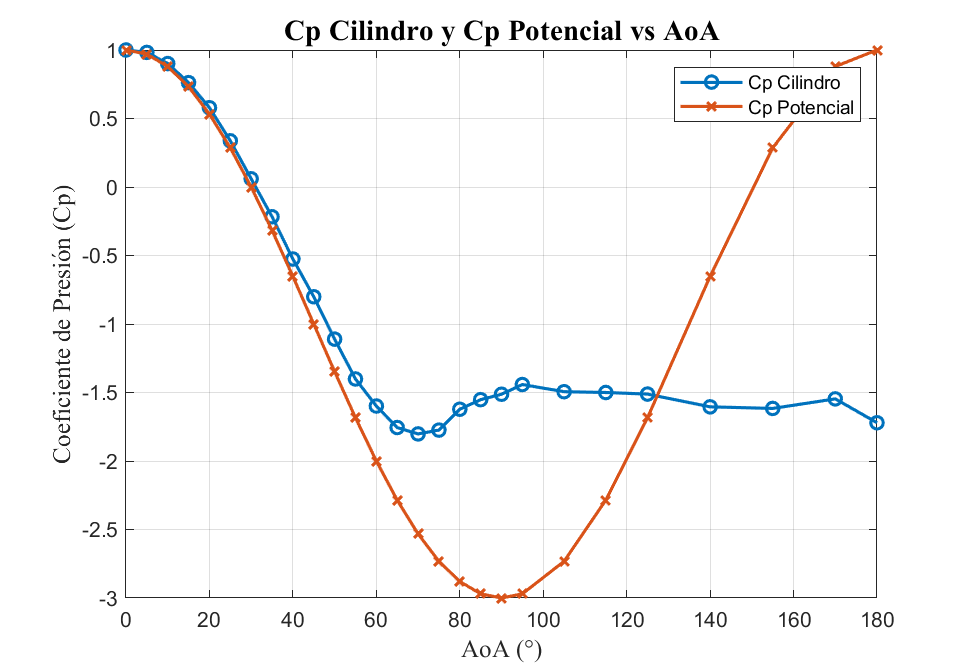
\includegraphics[width=0.9\textwidth]{01.Parte1/Figuras/Cilindro_Cp.png}
    \caption{Comparação entre o coeficiente de pressão do
experimento e o coeficiente de pressão potencial}
    \label{fig:Cp}
\end{figure}


\begin{figure}[htbp]
    \centering
    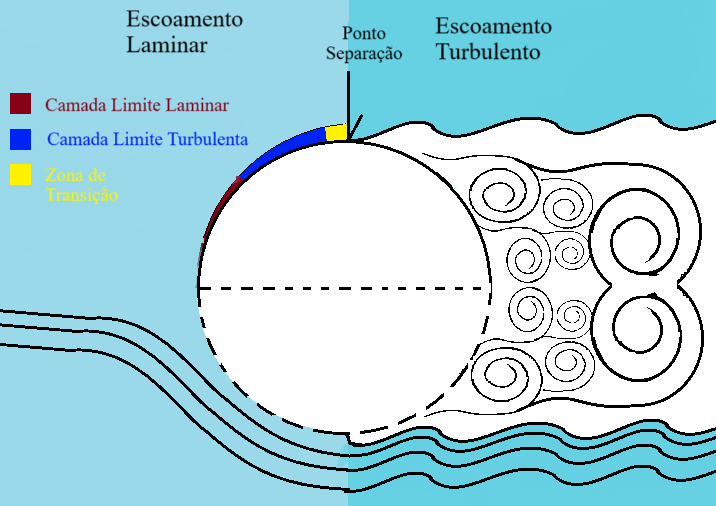
\includegraphics[width=0.9\textwidth]{01.Parte1/Figuras/Clindrof.png}
    \caption{Representação dos análises, adaptado de \cite{anderson2016introduction} - Figura 5.75, p. 402.}
    \label{fig:CilindroAnderson}
\end{figure}


\subsubsection{Desprendimiento de Fluxo}

 O fluxo é subsônico $ Mach = 0.05 \pm 1.9 \cdot 10^{-5} $. Como se evidencia, a separação do fluxo ocorre após os $88^\circ \pm 0.5^\circ$, um ponto onde o fluxo não consegue seguir a superfície do cilindro devido à queda de velocidade. Isso pode ser observado porque a inclinação da curva deixa de seguir o $C_P$ potencial e se torna aproximadamente constante.
\begin{equation}
   \frac{dC_{p}}{dAoA} = Cte ~~ ; ~~  C_P = -1.5 \pm 0.42
\end{equation}

% ----------------------------------------------------------------------

\subsubsection{Capa limite}
De $0^\circ \pm 0.5^\circ$ a $40^\circ \pm 0.5^\circ$ pode-se considerar laminar, uma vez que segue a linha de $C_P$ potencial (fluxo subsônico sem viscosidade), comparável a dizer que segue um fluxo que 'não possui fricção' na superfície. Experimentalmente, diz-se que é desprezível ao ter uma camada limite muito fina.


\begin{equation}
\begin{aligned}
\text{Laminar: } & \left| \frac{dC_{p}}{dAoA} - \frac{d\bar{C}_{p}}{dAoA_\infty} \right| = 0~~ ; ~~  -0.5 < C_P < 1\\ 
\text{Turbulento: } & \left| \frac{dC_{p}}{dAoA} - \frac{d\bar{C}_{p}}{dAoA_\infty} \right| > 0 ~~; ~~  -1.8 < C_P < -0.5 
\end{aligned}
\end{equation}


Depois de $40^\circ \pm 0.5^\circ$, temos uma transição para a camada limite turbulenta, pois a variação de $C_P$ é evidente. Geralmente, o fluxo turbulento tende a ser mais resistente ao desprendimento. Isso se deve ao fato de que, ao haver uma mistura mais eficaz de momento dentro da camada limite turbulenta, a influência da viscosidade do fluxo reduz sua velocidade (na superfície), levando a $C_P$ mais altos.

% -------------------------------------------------------------------------

\subsubsection{Transicion flujo Laminar a Turbulento}
A transição foi determinada a partir do ponto onde a velocidade do fluxo diminui abruptamente. O fluxo laminar apresenta uma queda mais suave na pressão à medida que o ângulo do cilindro aumenta.
    
\begin{equation}
   \text{Ponto Transição:}~  \frac{dC_{p}}{dAoA} = 0 ~~ ; ~~  C_P = -1.8 \pm 0.42
\end{equation}  


 Da Figura \ref{fig:Cp}, conclui-se que a transição ocorre aos $70^\circ \pm 0.5^\circ$. Para o caso deste experimento, considerou-se fluxo laminar para ângulos $<70^\circ$. Após a transição para fluxo turbulento, a mudança de $C_p$ é mais abrupta, embora se evidencie que o fluxo ainda consegue aderir à superfície do cilindro. A zona de fluxo turbulento está atrás do cilindro; isso se sabe ao concluir que o coeficiente de pressão atrás do cilindro $>100^\circ \pm 0.5^\circ$ se mantém constante, devido ao fato de que a velocidade do fluxo não muda.





% El desprendimiento de flujo ocurre en la región posterior del cilindro, donde el flujo no puede seguir la curvatura de la superficie debido a la caída de velocidad, lo que genera una zona de recirculación.

% El Cp se vuelve aproximadamente constante o deja de seguir la tendencia esperada a medida que el flujo se separa de la superficie. Este punto de desprendimiento suele estar alrededor de los 120°-150° medidos desde el frente (stagnation point) del cilindro.
% Transición de flujo laminar a turbulento:

% La transición ocurre antes del desprendimiento, cuando el flujo laminar se convierte en turbulento.
% En el gráfico de Cp, el flujo laminar muestra una caída más suave en la presión conforme se mueve desde la parte delantera hacia los costados del cilindro.
% Después de la transición a flujo turbulento, el descenso de Cp puede volverse más abrupto. Además, en la región de flujo turbulento, los valores de Cp pueden ser más bajos que en el flujo laminar, ya que el flujo turbulento puede adherirse más tiempo a la superficie del cilindro.
%Introduzir e inserir tabela com os dados
%Analisar e inserir gráfico de Cp

\subsection{Análise bidimensional na asa}
%Introduzir e inserir tabela com os dados
%Analisar e inserir gráficos de sustentação, arrasto e momento

\subsection{Análise tridimensional na asa}

\section{Conclusão}
\include{02.Parte2/Parte2}
\include{03.Parte3/Parte3}
\include{04.Parte4/Parte4}

%\section{Geral}
\label{sec: texto}

Boa documentação para \LaTeX \href{https://en.wikibooks.org/wiki/LaTeX}{\textit{ aqui}}.

\subsection{Texto}

\textbf{Negrito}.

\textit{Itálico}.

\underline{Sublinhado}.

\textsc{Small caps}.

\begin{bfseries}
Série de texto em negrito
\end{bfseries}

\hl{Texto grifado}

\begin{center}
Este texto está centralizado.
\end{center}

\subsubsection{Tamanho da Fonte}

\tiny
Muito pequeno

\scriptsize
Menos pequeno

\footnotesize
Rodapé

\small
Pequeno

\normalsize
Normal

\large
Maior

\Large
Grande

\LARGE
Muito grande

\huge
Extremamente Grande

\Huge
Enorme

\normalsize


\subsection{Espaçamentos}

\hspace{1cm}
\vspace{1cm}

\section{Listas}

\begin{itemize}
    \item Item normal
    \item [$\star$] Esse é um item com estrela.
    \item [a] Item com a
    \item [$\dagger$] Esse é um item com cruz.
\end{itemize}

\vspace{1cm}

\begin{enumerate}
    \item Esse é o primeiro nível.
    \begin{enumerate}
        \item Esse é o segundo.
    \end{enumerate}
\end{enumerate}

\section{Figuras e tabelas}
\label{sec: fig/tab}

\subsection{Figuras}

\begin{figure}[H]
    \centering
    \includegraphics[width=15cm]{figures/sample.png}
    \caption{Legenda}
    \label{fig: sample}
\end{figure}

\subsection{Tabelas}

Acesse esse \href{https://www.tablesgenerator.com}{\textit{link}} para fazer sua tabela.

\section{Matemática}

Seja $f$ a função $f(x)=x^2$.
Então $f(2)=4$ e \[ f(-3)=9. \]

\begin{equation}
    x = \frac{-b \pm \sqrt{b^2 - 4ac}}{2a}
\label{eq: bhaskara}
\end{equation}

\[ \alpha \delta \Delta \psi \]

\[ c_{l\alpha} \]

\[ \int_2^{15} x^2\,dx \]

\[ \left(\frac{1}{5}\right\}^6 \]

\[ \lim_{x \to 1} f(x) \]

\[ \sum_{i=1}^n i \]

\begin{align}
a^2 + b^2 &= c^2 \\
a+b &= c + 2
\end{align}

\begin{equation}
\begin{Bmatrix}
a & b\\
c & d
\end{Bmatrix}
\end{equation}

\begin{theorem}[Teorema de Pitágoras]
Em um triângulo retângulo, o quadrado da hipotenusa é igual à soma dos quadrados dos catetos.
\end{theorem}

\section{Referências Cruzadas}

Segundo a Equação \ref{eq: bhaskara}

Na Figura \ref{fig: sample}

Na Seção \ref{sec: texto}

\section{Citação}

Segundo Houghton \cite{houghton}

\begin{table}[H]
\centering
\caption{Valores calculados de módulo de impulso sofrido (I), energia cinética e quantidade de movimento (P).}
\label{tab:4}
\resizebox{\textwidth}{!}{%
\begin{tabular}{|c|c|}
\hline
Parâmetro    & Valor                \\ \hline
$\Delta t_1$ & $(0,094 \pm 0,001)s$ \\ \hline
$\Delta t_2$ & $(0,099 \pm 0,001)s$ \\ \hline
\end{tabular}%
}
\end{table}
%https://www.tablesgenerator.com

\bibliographystyle{plain}
\bibliography{Files_fixas/biblio}

\end{document}

